\section{Alternative Class Features}
Choosing a class fixes key aspects of a character: their role, their abilities, and their attack and save bonuses. However, you can change a class feature to provide a new experience. Variant versions of several of class features are presented below. If you prefer the variant to the standard class feature, ask your game master if he approves of your swapping out your class feature for the variant version.

These alternative class features can exist side by side with the standard class features---some bards might work alone while their comrades favor having contacts all over Athas---or can completely replace the standard features. The balance between the standard class features and the alternative features is up to the game master.

The description of alternative class features is the following.


\subsection{Class Name}
\subsubsection{Alternative Class Feature Name}
A general description of the ability.

\textbf{Special Requirement:} Any special requirements that you must meet before selecting the alternative class feature. Many of the alternative class features described here require ranks of a skill. Since skill ranks are purchased before class features are selected, you can meet this requirement at the same level that you gain the alternative class feature.

\textbf{Level:} The alternative class feature can be selected only at this level. In some cases, different levels might be given for different classes.

\textbf{Replaces:} The ability that you must sacrifice to gain the alternative class feature.

\textbf{Benefit:} The mechanical effects of the new ability.


\subsection{Bard}
\AlternateClassFeature{Contact}
{Instead of relying on their own wits like a traditional bard, a \emph{draqoman} relies on the help of others more capable in specific matters. Draqomen serve as guides and translators for newcomers to the cities. Local laws and customs vary by location, and a local resident who knows the city like the back of his hand and can call in a favor if necessary is definitely worth his pay. A draqoman will usually be loyal as long as he is paid and fed well. Mistreat your draqoman and you will soon find yourself on the wrong end of someone's blade or in the prisons run by the templars.}
{\skill{Diplomacy} 2 ranks, \skill{Gather Information} 4 ranks, \skill{Knowledge} (local) 4 ranks.}
{6th, 11th, and 16th.}
{You do not gain quick thinking, or its improvements at 11th and 16th levels.}
{
	You gain the trust of two non-player characters he can rely on when the time comes. You can ask for a favor once per week per contact. Contacts come in three varieties, one of which you must choose: influence contacts, skill contacts, and trade contacts (see \hyperref[sec:contacts]{Contacts}).

	You gain one additional contact every three levels thereafter (3 at 9th, 4 at 12th, 5 at 15th, and 6 at 18th level).
}
\AlternateClassFeature{Procurer}
{To all outward appearances, procurers seem to be everyday elf traders. They conduct their thefts in secret, using normal trading practices to cover their filching activities. These elves usually work for elven merchant houses, filling the market stalls with goods stolen from other merchants, nobles, free citizens, templars, and even the sorcerer-kings.}
{Elf or half-elf.}
{4th, 8th, 12th, 16th, or 20th.}
{You do not gain a trade secret.}
{
	You gain +5 in \skill{Search} checks to find secret doors, and if you pass within 1.5 meter of a secret door, you are entitled to a \skill{Search} check to notice it as if the character was actively looking for it.
}


\subsection{Fighter}
\AlternateClassFeature{Reckless}
{The eagle knights are among the most brutal and fanatical Draji warriors. They are more than willing to charge headfirst into battle for the glory of Draj and their god-king.}
{Must be trained by the Draji army.}
{11th.}
{You do not gain martial prowess.}
{
	When using the attack or full attack option, you can subtract a number from his Armor Class and add this number to damage inflicted on successful attacks. This number may not exceed your base attack bonus. The Armor Class penalty and damage bonus last until the your next standard action.
}
\AlternateClassFeature{Savage Hunter}
{The savage hunter is the most common elf warrior type, serving as both a tribal defender and an important food provider. Respected by others of the tribe, the savage hunter uses the same skills to hunt prey and to fight outsiders and other threats to the tribe. The ways of the city-states are alien to these wilderness warriors, for they are only at home in the wastes when on a hunt.}
{Elf or half-elf.}
{1st.}
{You do not gain a bonus feat.}
{
	You gain \feat{Track} as a bonus feat. You add \skill{Survival} to your fighter class skills.
}

\AlternateClassFeature{Tik-Tik}
{Larger and less dexterous than most other kreen, the ``hunter-of-hunters'' guards the weaker members of the pack. In dangerous territory, Tik-Tik rarely hunt, unless the pack's normal hunters are spread too thinly or have been incapacitated by enemies.}
{Thri-kreen.}
{1st.}
{You do not gain a bonus feat.}
{
	Your natural armor bonus increases by 1 (+3 total). You add \skill{Survival} to your fighter class skills.
}


\subsection{Gladiator}
\AlternateClassFeature{Flexibility Adjustment}
{These gladiators adjust their armor to improve their reflex capabilities instead of increasing the area it protects.}
{}
{5th, 10th, 15th, and 20th.}
{You do not gain armor optimization, or its improvements at 10th, 15th, and 20th levels.}
{
	You improve the maximum Dexterity bonus and reduce the armor check penalty by 1, whenever you are wearing any armor you are proficient with.

	At every five levels thereafter, the improvement increases by 1 (2 at 10th, 3 at 15th, and 4 at 20th level).
}
\AlternateClassFeature{Lighten Load}
{By changing slightly the armor to their own bodies, these gladiators can move faster with a heavier armor.}
{}
{5th.}
{You do not gain the first armor optimization.}
{
	You treat the armor as one category lighter (e.g. medium armor is treated as light armor), whenever you are wearing any armor you are proficient with.
}


\subsection{Psion}
\AlternateClassFeature{Contact}
{The cities of Athas are filled with intrigue, treachery, and double-dealing. In this setting, information is a weapon that may be wielded against one's enemies. The auditor's job description ranges from information broker to psionic assassin. In most cities, the templars have auditors working for them. Other auditors are members of the Veiled Alliance, criminal gangs, or are employed by the merchant dynasties.}
{\skill{Diplomacy} 2 ranks, \skill{Gather Information} 4 ranks, \skill{Knowledge} (local) 4 ranks.}
{1st, 5th, 10th, 15th, and 20th.}
{You do not gain any bonus feat.}
{
	You gain the trust of a non-player character he can rely on when the time comes. You can ask for a favor once per week per contact. Contacts come in three varieties, one of which you must choose: influence contacts, skill contacts, and trade contacts (see \hyperref[sec:contacts]{Contacts}).

	You gain one additional use of contact at 5th level and every four levels thereafter (2 contacts at 5th, 3 at 9th, 4 at 13th, 5 at 17th).
}
\AlternateClassFeature{Psionic Ritual}
{Bereft of formal training in the Way, psionically talented individuals from the tribal and nomadic peoples of the Tablelands and beyond must make do with their own understanding of the psionic arts. Seen by formally trained psions as an aberration of proper psionic practice, these self trained individuals can sometimes produce effects that leave their detractors speechless.}
{\skill{Profession} (herbalist) 8 ranks, \skill{Survival} 6 ranks.}
{10th.}
{You do not gain a bonus feat.}
{
	Once per day, you can perform such a ritual to temporarily increase your Will. Each psionic ritual is unique, being of your own design, but all take one hour to complete and require a DC 20 \skill{Concentration} check. If the ritual is successful, you gain 1d4+1 temporary power points over and above your normal maximum. These power points remain available for one day or until they are used.
}
\begin{figure*}[t!]
\centering
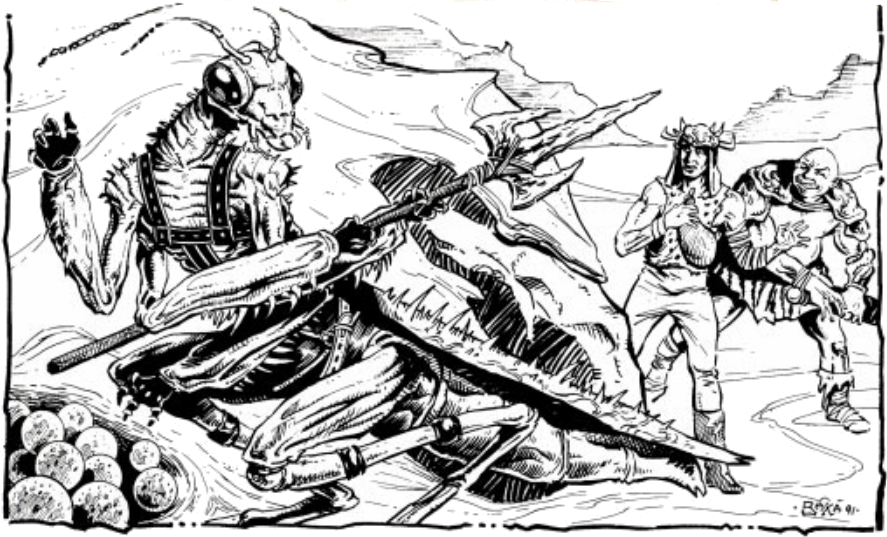
\includegraphics[width=\textwidth-1cm]{images/thrikreen-1.png}
\WOTC
\end{figure*}
\AlternateClassFeature{Tekchakak}
{The tekchakak is devoted to the preservation and prosperity of clutch and pack. These psionicists use their abilities to support their clutchmates and packmates, helping to find prey and to defend compatriots against raiders and predators. Within a
thri-kreen pack, the tekchakak offers advice, guidance, and teaching in addition to active support through their psionic abilities.}
{Thri-kreen.}
{1st.}
{You do not gain a bonus feat.}
{
	You no longer have alien mind (see \chapref{Character Races}). You add \skill{Survival} to your psion class skills.
}


\subsection{Ranger}
\AlternateClassFeature{Desert Runner}
{Desert runners are elves that have devoted themselves to the run, pushing themselves to the limit of Elven running ability. They are the scouts and messengers of a tribe. They run ahead of the rest, or alone through the desert to deliver important messages or items between clans with the greatest of speed. They are also some of the more competent hunters of the tribe able to track quarry silently while moving quickly through the desert.}
{Elf or half-elf.}
{4th.}
{You do not gain an animal companion.}
{
	You gain +1 bonus per ranger level on all \skill{Concentration} checks related to the elf run ability, and all other checks to continue running. This includes skill checks to avoid tripping or falling and saving throws to resist effects that would directly slow or impede movement (such as a Will save to resist a \spell{slow} spell). It does not however include indirectly related checks, such as a \skill{Spot} check to notice a pit trap.

	You gain +3 meters of land speed while wearing no armor or light armor, and not carrying heavy load. Your speed increases by 3 meters for every three ranger levels thereafter (+6 m at 7th, +9 m at 10th, +12 m at 13th, +15 m at 16th, and +18 m at 19th).

	You gain +1 AC dodge bonus when running. This bonus increases by 1 for every three ranger levels thereafter (+2 at 7th, +3 at 10th, +4 at 13th, +5 at 16th, and +6 at 19th).

	\emph{Desert runner} is a psi-like ability.
}
\AlternateClassFeature{Elf Favored Enemy}
{These insectoid hunters love the taste of elf flesh, and they prey upon the desert runners whenever the  opportunity presents itself. In order to combat the threat posed by the fast, strong, and cunning thri-kreen, a special class of desert runner has developed---the thri-kreen slayer.}
{Elf or half-elf.}
{1st.}
{You do not gain favored enemy.}
{
	You narrow down your choice of favorire enemy to thri-kreen. You gain a +3 bonus on \skill{Hide}, \skill{Listen}, \skill{Move Silently}, \skill{Spot}, and \skill{Survival} checks when using these skills against creatures of this race. Likewise, you get a +3 bonus on weapon damage rolls against such creatures.

	Each time you gain a new favored enemy and you choose to increase your bonus against thri-kreen, it increases by 3.
}
\AlternateClassFeature{Salvage}
{The kik has fully turned away from the life as a hunter and instead embraced the life of a raider, known in the language of the thri-kreen as a kik. The kik are in many ways more barbaric then the average kreen who roam the Tablelands, though they are not as feral as their cousins the trin.}
{Thri-kreen, \skill{Search} 5 ranks, \skill{Survival} 5 ranks.}
{7th.}
{You do not gain woodland stride.}
{
	You can make a \skill{Search} check to salvage destroyed caravans and vehicles. If the check succeeds, you earn ceramic pieces by the amount indicated on \tabref{Salvage Vehicle}, either by selling the salvaged parts or using them to offset the cost of other items.

	A particular vehicle can be successfully salvaged only once. Any further attempts to salvage the wreckage fail automatically.

	\Table{Salvage Vehicle}{Xccc}{
	\tableheader Vehicle Size & \tableheader Time & \tableheader \skill{Search} DC & \tableheader cp Earned\\
	Large or smaller & 15 min. & 10 & 10\\
	Huge & 30 min. & 15 & 20\\
	Gargantuan & 1 h & 20 & 30\\
	Colossal & 3 h & 25 & 40\\
	}
}
\AlternateClassFeature{Sand Chitin}
{Usually selected from those thri-kreen that are slightly smaller and quicker, these kreen are trained extensively in the lore of the hunt and the way of stealth, honing their natural skills beyond those of the norm of their kind.}
{Thri-kreen.}
{1st.}
{You do not gain wild empathy.}
{
	Your racial \skill{Hide} bonus increases by 2 (+6 total). For every four ranger levels thereafter, it increases by another 2 (+8 at 5th, +10 at 9th, +12 at 13th, and +14 at 17th).
}


\subsection{Rogue}
\AlternateClassFeature{Arcane Assassin}
{Wizards are target of many assassinations, either by the demands of the Veiled Alliance targeting defilers or by the templarate targeting the veiled ones. Arcane assassins know how to put their foes under stress and don't waste any opportunity to strike.}
{\skill{Knowledge} (arcane) 6 ranks, \skill{Spellcraft} 6 ranks, \skill{Spot} 10 ranks.}
{10th, 13th, 16th, or 19th.}
{You do not gain an special ability.}
{
	Any spellcaster the rogue is flanking provokes an attack of opportunity if they try to cast defensively. The spellcaster knows of this limitation.
}
\AlternateClassFeature{Death Attack}
{The Shadows are a mysterious elf tribe of which legends and bard's tales are spun. This secretive network of elves specializes in covert and illegal operations---espionage, assassination, extortion, theft, smuggling and black market trading, to name a few. References of the shadows go back hundreds of years, and some claim they have always been around.}
{Elf, any Evil alignment, \skill{Disguise} 4 ranks, \skill{Hide} 4 ranks, \skill{Spot} 6 ranks.}
{3rd.}
{You do not gain trap sense.}
{
	If a rogue studies her victim for 3 rounds and then makes a sneak attack with a melee weapon that successfully deals damage, the sneak attack has the additional effect of possibly either paralyzing or killing the target (rogue's choice). While studying the victim, the rogue can undertake other actions so long as her attention stays focused on the target and the target does not detect the rogue or recognize the rogue as an enemy. If the victim of such an attack fails a Fortitude save (DC 10 + \onehalf the rogue's class level + the rogue's Int modifier) against the kill effect, he dies. If the saving throw fails against the paralysis effect, the victim is rendered helpless and unable to act for 1d6 rounds plus 1 round per level of the rogue. If the victim's saving throw succeeds, the attack is just a normal sneak attack. Once the rogue has completed the 3 rounds of study, she must make the death attack within the next 3 rounds.

	If a death attack is attempted and fails (the victim makes his save) or if the rogue does not launch the attack within 3 rounds of completing the study, 3 new rounds of study are required before she can attempt another death attack.
}


\subsection{Templar}
\AlternateClassFeature{Badna's Chosen}
{Templars of Raam have been told that their divine powers stem from an entity called Badna. Most templars know or at least suspect that Badna is a fictional being created by Abalach-Re to suppress the people of Raam.}
{\skill{Knowledge} (religion) 5 ranks, must be from the templarate of Raam.}
{8th.}
{To select this class feature, you must permanently sacrifice one of your 4th-level spell slots.}
{
	You always act in the surprise round, but you permanently lose 2 points of Wisdom.
}
\AlternateClassFeature{Hamanu's Intervention}
{Urikite templars wear yellow robes, and as they rise in status strands of metal are woven into their sleeves and they receive Hamanu's personal attention. Under the tutelage of Hamanu, his templars excel in the art of combat and they can call upon their liege to power their magic or blows.}
{\skill{Knowledge} (warcraft) 4 ranks, must be from the templarate of Urik.}
{6th or any even-numbered higher level.}
{To select this class feature, you must permanently sacrifice one of your 3rd-level spell slots.}
{
	Once per day, as a move action, you may choose between +4 bonus on caster level to the next spell you cast or make your next melee attack an automatic threat (roll to determine if the attack is a critical hit).

	You may select this ability multiple times. Each time you must sacrifice another 3rd-level spell slot.

	\emph{Hamanu's intervention} is a spell-like ability.
}
\AlternateClassFeature{Nibenay's Diligence}
{The Nibenese templarate consists of women, all wedded to the Shadow King. Disciplined, educated and trained in the arts of war, the templar-wives fit perfectly into Nibenay's highly autocratic structured system of government.}
{\skill{Knowledge} (warcraft) 5 ranks, must be from the templarate of Nibenay.}
{8th.}
{To select this class feature, you must permanently sacrifice one of your 4th-level spell slots.}
{
	You can take 10 on \skill{Concentration} checks to cast spells defensively.
}
\AlternateClassFeature{Oba's Truth}
{The disciples of the Oba follow their own rites and traditions that are as ancient as those of the people of Gulg. Lalali-Puy's templars  The queen allows for templars to be dispatched to a residential dagada at the request of the dagada's leader. This request usually comes when an ambo is fearful for the security of his dagada or suspicious of an illegal activity, such as smuggling or magic use.}
{\skill{Knowledge} (nature) 7 ranks, must be from the templarate of Gulg.}
{10th.}
{To select this class feature, you must permanently sacrifice one of your 5th-level spell slots.}
{
	Once per day, you may poison a creature with a touch attack. That creature becomes infused with poison for 24 hours. If the creature tells a lie, it suffers the effect of the poison with no saving throw. The initial damage is 2d6 Con, and the secondary damage is 1d6 Con. Casting \spell{neutralize poison} or \spell{heal} will remove the poison from the victim's body.

	\emph{Oba's truth} is a spell-like ability.
}
\AlternateClassFeature{Ral's Convergence}
{For more than a thousand years, the moon priests have served Tectuktitlay, the king of Draj. Dressed in blue robes, with a yellow moon in front and in the back of their robes, the Moon Priests are responsible for the administration of the Temples of Ral and Guthay, as well as being the lead organizers of the sacrifices on the Great Pyramid.}
{\skill{Knowledge} (nature) 5 ranks, must be from the templarate of Draj.}
{8th.}
{To select this class feature, you must permanently sacrifice one of your 4th-level spell slots.}
{
	Once per day, you may reroll one d20 roll that they have just made. You must keep the result of the second roll, even if it's worse than the original roll.

	\emph{Ral's convergence} is a spell-like ability.
}

% Tyr
% Balic
% Kurn
% Eldaarich


% \AlternateClassFeature{Bureau Specialization}
% {}
% {Must be from the templarate of Tyr.}
% {8th and 12th.}
% {To select this class feature, you must permanently sacrifice one of your 4th-level spell slots, then another 6th-level spell slot at 12th level.}
% {Choose a templar class skill. You gain +3 bonus on checks of the chosen skill at 8th level.

% At 12th level, this bonus increases to +6 and you can take 10 even if stress and distraction would normally prevent you from doing so.}


% \subsection{Wilder}
% \AlternateClassFeature{Psionic Ritual}
% {Bereft of formal training in the Way, psionically talented individuals from the tribal and nomadic peoples of the Tablelands and beyond must make do with their own understanding of the psionic arts. Seen by formally trained psions as an aberration of proper psionic practice, these self trained individuals can sometimes produce effects that leave their detractors speechless.}
% {\skill{Profession} (herbalist) 4 ranks, \skill{Survival} 4 ranks.}
% {7th.}
% {You do not improve wild surge at 7th level. Instead, you gain wild surge +3 at 11th level, with an addtional increase of +1 every four levels there after (to a maximum of +5 at 19th level).}
% {
% 	Once per day, you can perform such a ritual to temporarily increase your Will. Each psionic ritual is unique, being of your own design, but all take one hour to complete and require a DC 20 \skill{Concentration} check. If the ritual is successful, you gain 1d4+1 temporary power points over and above your normal maximum. These power points remain available for one day or until they are used.
% }


\subsection{Wizard}
\AlternateClassFeature{Exegete}
{As a result of their endless research and studies, arcanists end up knowing a little about a lot of different things. They are consulted often, becoming experts and advisers for their tribes.}
{Elf, \skill{Knowledge} (history) 10 ranks.}
{10th.}
{You do not gain a bonus feat.}
{
	You are considered to be trained in all forms of Knowledge and can choose to take 10 in \skill{Knowledge} checks which you have at least 10 ranks in.
}

\begin{figure*}[t!]
\centering
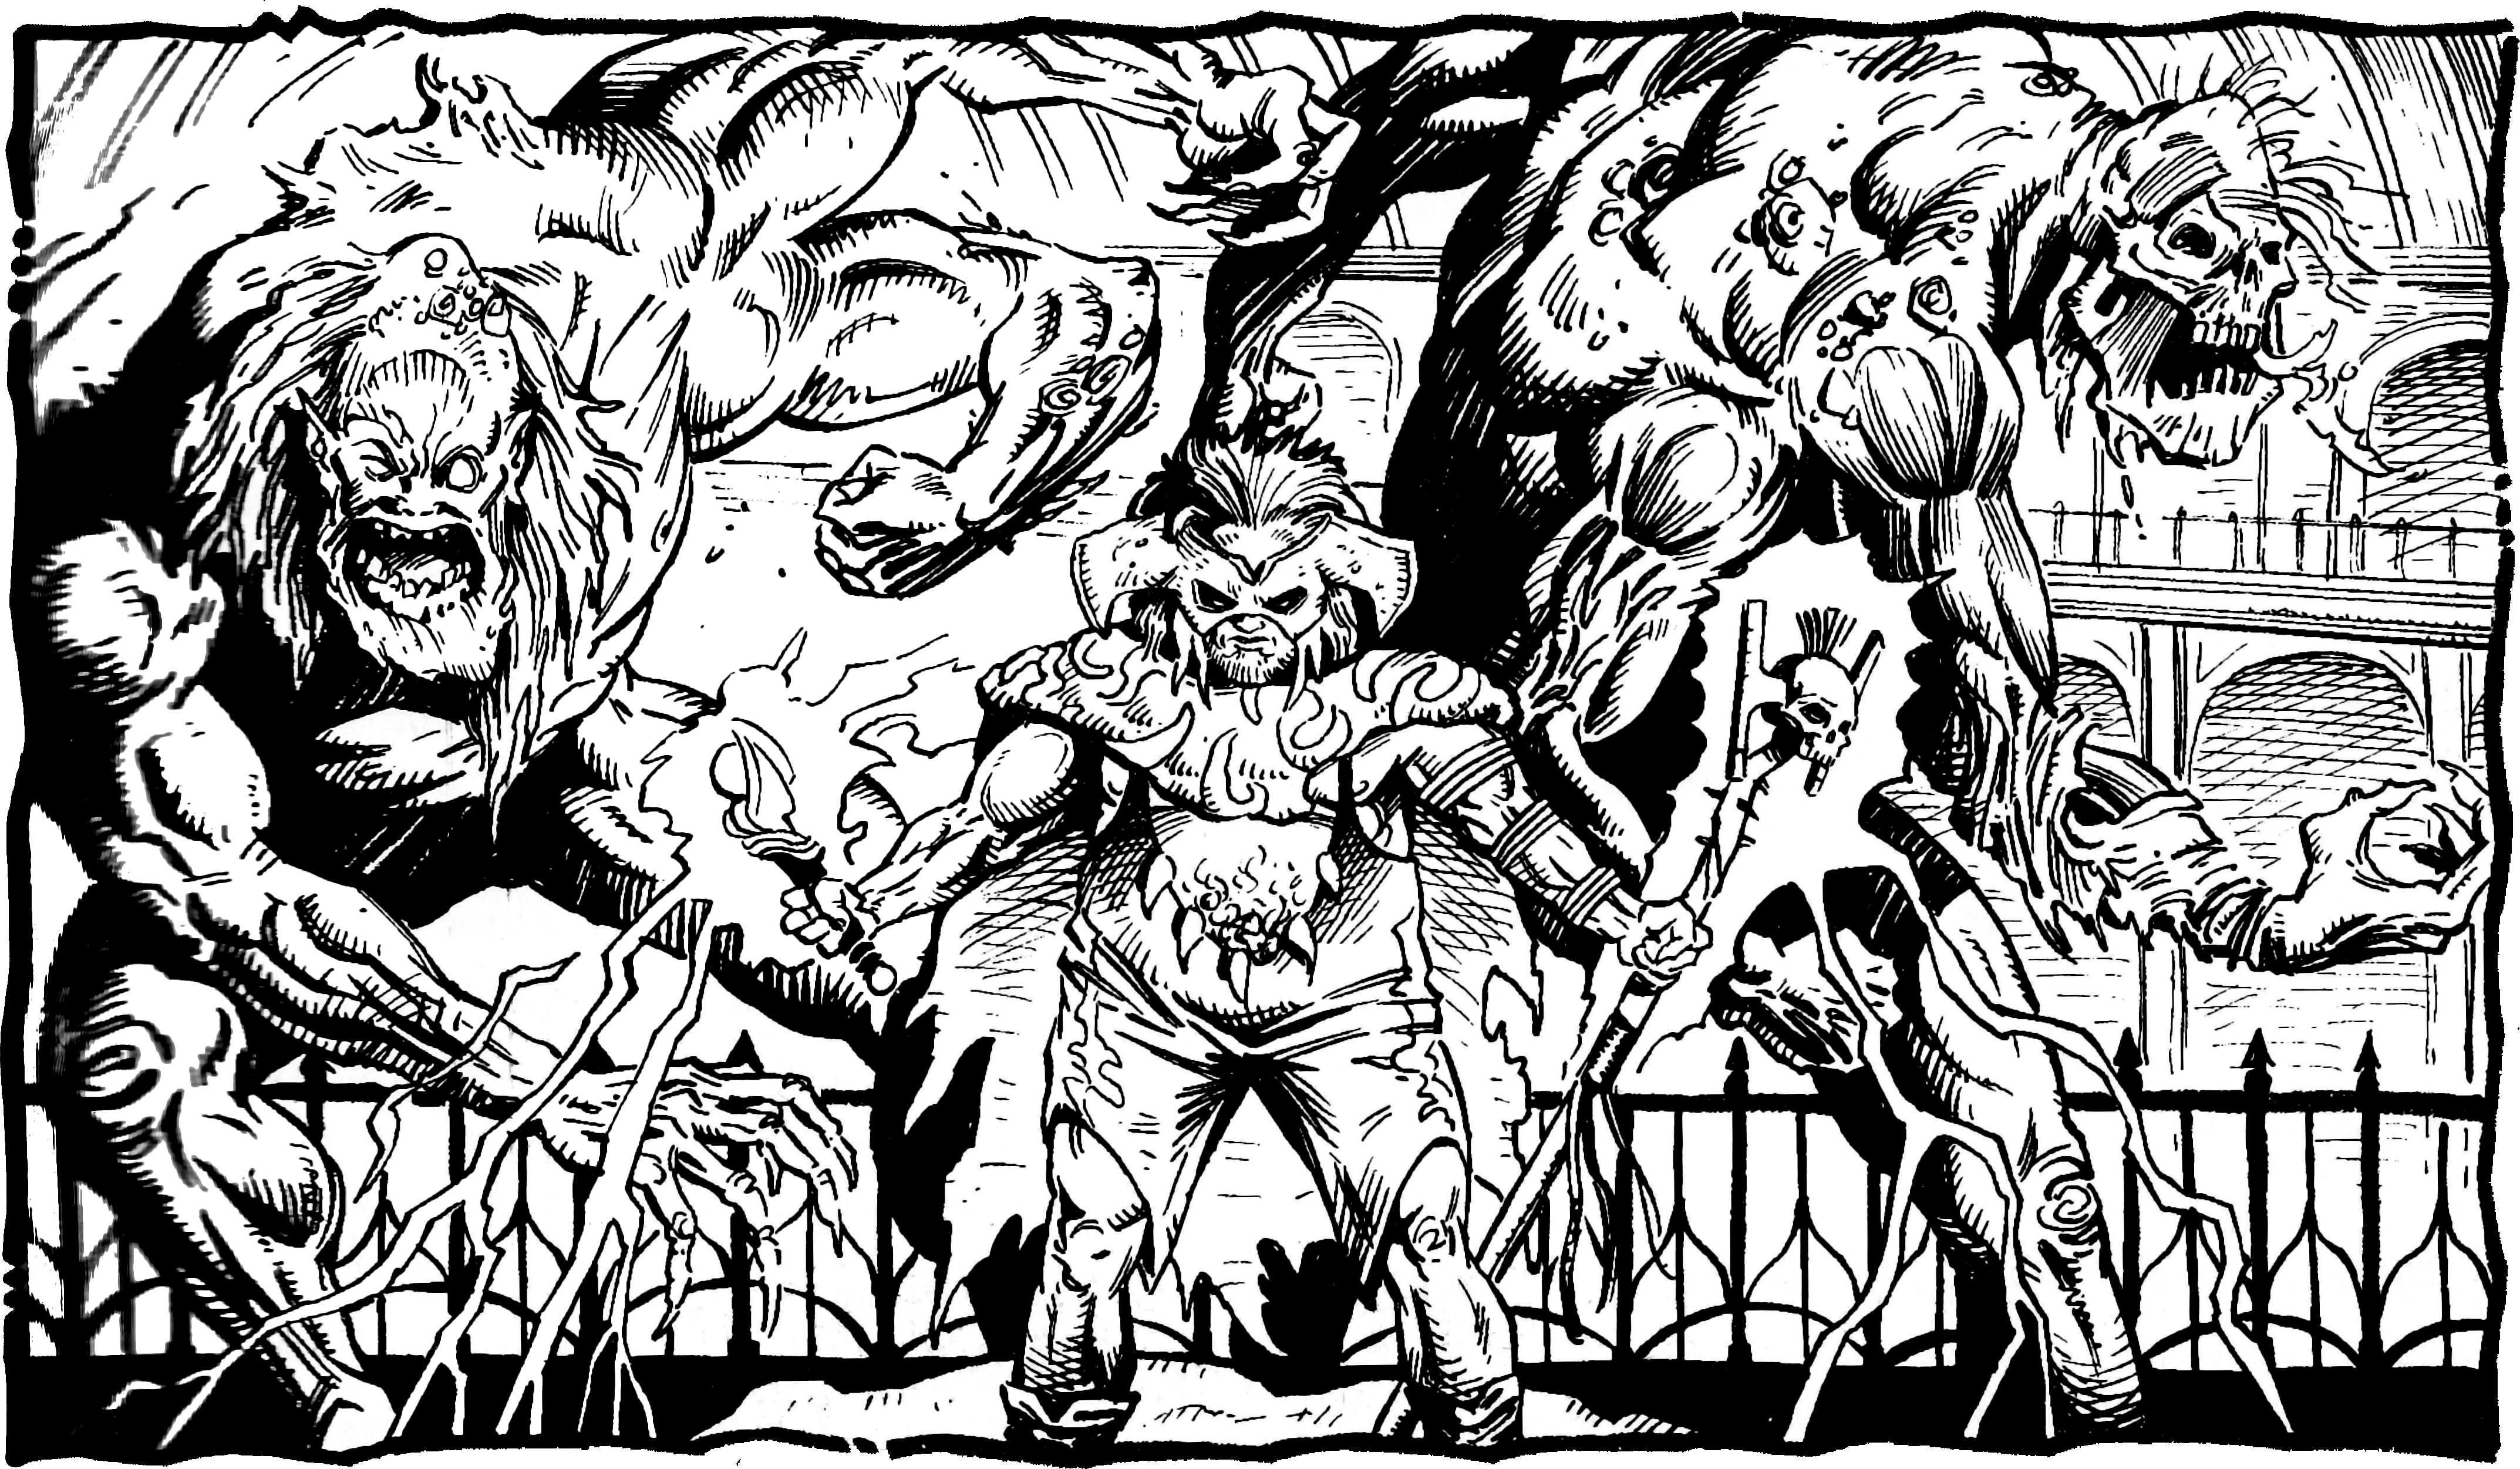
\includegraphics[width=\textwidth]{images/necromancer-1.png}
\WOTC
\end{figure*}
\AlternateClassFeature{Phantasmal Guardian}
{Halfling protectors are masters of illusions that can aid their tribes and bring doom to their enemies in many strange ways.}
{Halfling, \skill{Knowledge} (nature) 10 ranks, \skill{Spellcraft} 10 ranks.}
{10th.}
{To select this class feature, you must permanently sacrifice one of your 5th-level spell slots.}
{
	You can summon a non-corporeal shadow figure that wards an area with a radius of 30 m + 3 m per level. Any other creature entering the warded area, except you and those you designate, will be attacked by the \emph{phantasmal guardian}, as per the \spell{phantasmal killer} spell. The \emph{guardian} can only attack once, where upon it dissipates. Summoning the \emph{guardian} takes 1 minute, and it remains in the area until you dispels it (move action, unlimited range), or until it attacks someone. You can only have one \emph{guardian} summoned at a time.

	You can use this ability 3 times per day.

	\emph{Phantasmal guardian} is a spell-like ability.
}
% \AlternateClassFeature{Psionic Mimicry}
% {The arena mage is a wizard who has acquired the skills necessary to survive the rigors of arena combat, engaging his opponents with an arsenal of spells. The lesson to conceal this spellcasting ability comes quickly, as failure means death. As such, an arena mage becomes a
% master at casting spells in secret, as well as masking his magic-use. To accomplish this feat, the arena mage has developed a unique talent to help him: giving his spells the trappings of psionic powers. Through the art of deception and a constant charade of psionic aptitude he is able to maintain secret his spellcasting even in the most public of places.}
% {\skill{Bluff} 4 ranks, \skill{Concentration} 4 ranks, \skill{Disguise} 4 ranks, \skill{Knowledge} (psionics) 4 ranks.}
% {1st.}
% {You do not gain a familiar.}
% {
% 	% You may attempt to conceal the fact that you are attempting to cast a spell. This is an especially important skill for wizards, who are all-too-frequently the unfortunate target of impromptu lynch mobs.
% 	When fighting in an gladiatorial arena, you may disguise your spells as psionic powers by making a \skill{Bluff} check as a move action, to distract the crowd. Spells with psionic counterparts, such as \spell{daze}, emulate the displays of their counterparts. Spells without psionic counterparts get attributed random displays.

% 	Onlookers may oppose the roll with a \skill{Sense Motive} or \skill{Spellcraft} check. If the spell being cast has a psionic counterpart, they may also oppose with a \skill{Psicraft} check.

% 	Defilers with this ability are accustomed to minimizing their damage in an arena and do not suffer additional penalties.
% }
\AlternateClassFeature{Rebuke Undead}
{Necromants are wizards draw their power from the undead plane known as the Gray, instead of the plant life. They are seeking to unravel the mysteries of death and find answers to questions that only the ancient dead know.}
{You must be a specialist necromancer, \skill{Knowledge} (arcana) 6 ranks, \skill{Knowledge} (religion) 6 ranks.}
{5th.}
{You do not gain a bonus feat.}
{
	You gain the supernatural ability to rebuke undead. You may use this ability a number of times per day equal to 3 + your Charisma modifier. You rebuke undead as a cleric four levels lower would.
}